\chapter{Implementation of an IoT based Electronic Voting Machine}

\section{Hardware Reference}

\begin{table}[h!]
    \centering
    \begin{tabular}{|l|c|p{5cm}|}
        \hline
        \textbf{Basic Component List} & \textbf{Number} & \textbf{Notes} \\
        \hline
        NodeMCU ESP32  & 1 & Development board for prototyping \\
        \hline
        1,8" LCD Display Module  & 1 & 128x160 Pixel, ST7735R (Display Driver), includes microSD Slot \\
        \hline
        Button module with 2 Buttons & 1 & For interacting \\
        \hline
		Jumper Wires Female to Male & 22 & For connecting components \\
        \hline
        Breadboard & 1 & For building circuits \\
        \hline
    \end{tabular}
    \caption{Basic Component List for Guardian Prototype}
    \label{tab:basic-component-list}
\end{table}

\begin{figure}
	\centering
	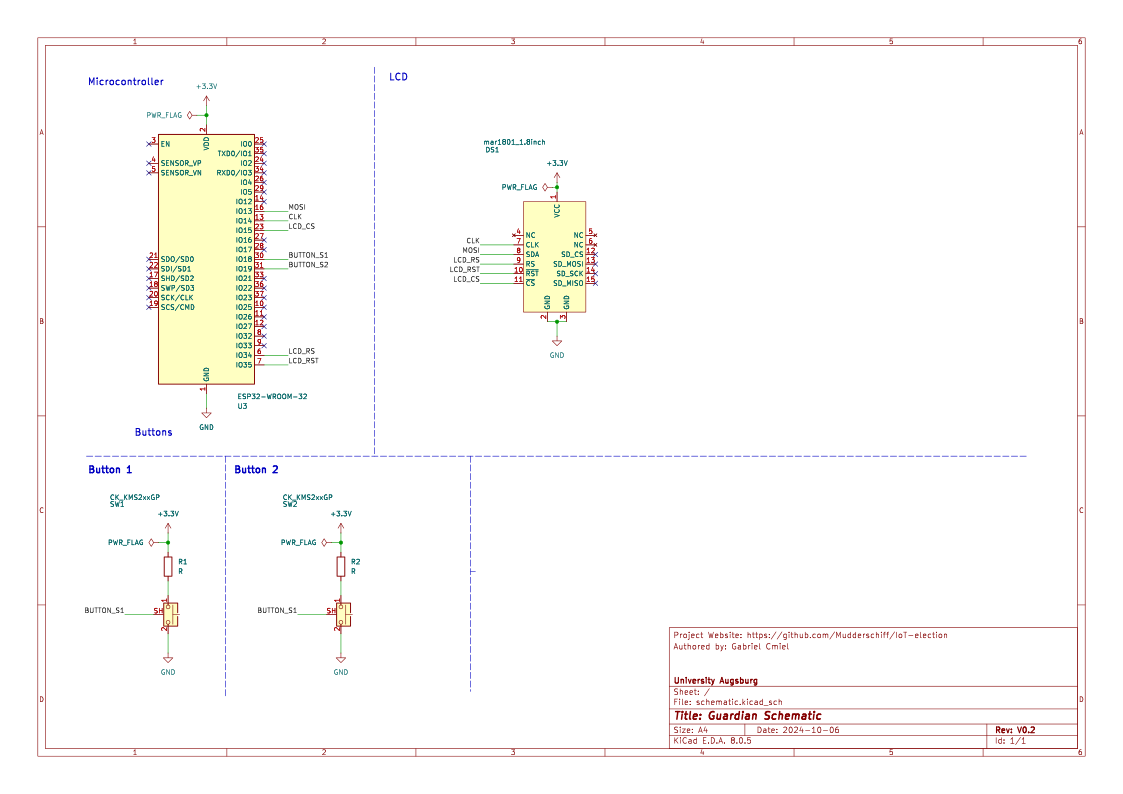
\includegraphics[scale=.5]{abbildungen/schematic.png}
	\caption{Schematic of the Guardian Prototype}
	\label{Fig:schematic}
\end{figure}

As shown in Table \ref{tab:basic-component-list}, the hardware components used in our prototype include a ESP32 development board, an LCD display module, jumper wires, breadboard and a module with 2 Buttons. The connectivity of these components are shown in the schematic in Figure \ref{Fig:schematic}. The NodeMCU ESP32 development board is used as the Main Controller. The LCD display module is used to display information to the user. The button module is used to interact with the user. The jumper wires are used to connect the components. The breadboard is used to build the circuits.

\subsection{NodeMCU ESP32 Development Board}
The NodeMCU ESP32 development board is equipped with the ESP32-WROOM-32 module. The ESP32-WROOM-32 module could therefore be replaced by the newer ESP32-WROOM-32E module. The ESP32-WROOM-32E module uses a ESP32-D0WD-V3 or ESP32-D0WDR2-V3 chip which are based on chip revision v3.0 or v3.1 which fixes some Hardware bugs \cite[1]{esp32-module-new}, \cite[11]{esp32-series}, \cite[3-4]{esp32-errata}. 

\begin{comment}
    “The ESP32-D0WD-V3 chip has checks in ROM which prevent fault injection attack” – Espressif Security Advisory
\end{comment}


\subsection{1,8" LCD Display Module}
The 1,8" LCD Display Module has a resolution of 128x160 Pixels and is equipped with a ST7735R Display Driver.  The module also contains a microSD Slot which won't be used in this project \cite[2]{lcd}.
The ESP-IDF component lvgl_esp32_drivers


\subsection{Button Module}
The Button Module is an integrated circuit that features 2 buttons and integrated pull-up resistors. \cite[1]{button-ds}

\section{Python Client}
Our python client imports the python package ElectionGuard \cite{python-reference}. The ElectionGuard Python package is a reference implementation of the ElectionGuard 1.0 specification. It covers the entire suite of functionality required to implement an end-to-end verifiable election as part of a voting system \cite{eg-docs}. 



In the proposed voting system the python client will act as the administrator, the ballot box and the encryption device of the election. Administrating the election requires loading and semantically verifiying the Election manifest before the election.





Before the election the python client load the Election Manifest for our election and semantically checks the data format required to conduct an ElectionGuard Election. 




The python client loads the manifest file used for our election. In ElectionGuard an election manifest has to be semantically checked against the data format required to conduct an ElectionGuard Election. 


The python client then generates the election keys and the election context. The election keys are used to encrypt the ballots and the election context is used to verify the election. The python client then encrypts the ballots and generates the proofs of the encryption. The encrypted ballots and the proofs are then sent to the ESP32. The ESP32 decrypts the ballots and verifies the proofs. The ESP32 then generates the proofs of the decryption and sends them back to the python client. The python client then verifies the proofs of the decryption and generates the proofs of the election. The proofs of the election are then sent to the ESP32. The ESP32 verifies the proofs of the election and sends the results back to the python client. The python client then verifies the results and outputs the final results of the election.

The tasks of the python client can be divided into three stages pre-election, intra-election and post-election.







The python client loads the manifest file used for our election. In ElectionGuard an election manifest has to be semantically checked against the data fromat required to conduct an ElectionGuard Election.



Espressif IoT Development Framework (ESP-IDF) is a software development framework intended for the development of Internet-of-Things (IoT) applications for the ESP32 board \cite{esp-prog}. ESP-IDF consists of components written specifically for ESP-IDF as well as third-party libraries.\cite{esp-prog} For example, the real-time operating system kernel used for ESP-IDF applications is the third-party component called FreeRTOS \cite{esp-prog}. ESP-IDF projects use the same componment based approach and can be seen as an amalgamation of a number of components \cite{esp-prog}.

\begin{figure}
	\centering
	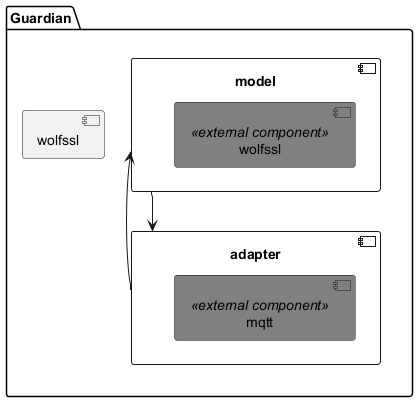
\includegraphics[width=1\textwidth]{abbildungen/Diagramme/components.png}
	\caption{}
	\label{Fig:uml-classes-python}
\end{figure}


\section{Computation}
ElectionGuard uses integer ElGamal within specific cryptographic equations. Four operation are performed - all on very large integer values. These operations are modular exponentiation, modular multiplication, modular addition, and SHA-256 hash computation. These operations can be performed by either importing specialiced tools to perform these large integer operations, or by implementing these operations from scratch. When implementing the modular operations from scratch, intermediate values can get excessively large often times it is necessary to perform special methods such as modular reduction to keep the values within a reasonable range \cite[21, 25-26]{eg-spec}. The modular exponentiation operation imposes the highest computational cost among all computations and is the limiting factor in any performance analysis. \cite[22]{eg-spec}. Using fast libraries for modular arithmetic is thus crucial to achieve good performance \cite[22]{eg-paper}.

\subsection{Cryptographic constants}
Most exponentiations in ElectionGuard have a fixed base, either the generator g or the election public key K. \cite[22]{eg-paper}. Generator G is one of the cryptographic constants predefined in the ElectionGuard specification. With standard baseline we have a 4096-bit prime p, a 4096-bit generator g, and a 256-bit prime q. With reduced parameters we have a 3072-bit prime p, a 3072-bit generator g, and a 256-bit prime q. \cite[21-23]{eg-spec}. In this application we use the reduced parameters as they offer a better performance although at a lower security level \cite[36-37]{eg-spec}.


\subsection{Comparison of ElectionGuard Implementations}
 The Python reference implementation of ElectionGuard uses the C-code Gmpy2 library for large integer arithmetic. \cite{eg-docs}. \cite{esp32-ref} The C++ and Kotlin implementations of ElectionGuard uses HACL* C library for cryptographic primitives. \cite{eg-docs}. Furthermore, the C++ implementation also uses pre-computed tables to speed up some modular exponentiations \cite{eg-docs}. This is possible because most exponentiations have a fixed base, either the constant generator or the election public key. The pre-computed tables contain certain powers of these bases. \cite{eg-docs}.

\subsubsection{Feasability of the Python reference on ESP32}
It could be possible to run the python reference on the ESP32 using Micropython. Micropython is an implementation of Python 3.x targetting microcontrollers and embedded systems. Functionalities of the python standard library are mirrored and "micro-ified" to fit with the limitations of microcontrollers such as memory and speed \cite{micropython} \cite[234]{micropython-performance}. Apart from python the electionguard python reference requires the C-coded python library Gmpy2 for large integer arithmetic \cite{eg-ref}. Disadvantages of this approach is that some needed modules, functions and classes may be missing from Micropython. \cite{micropython}. Furthermore, MicroPython applications suffer from memory fragmentation and objects that grow in size \cite[234]{micropython-performance}. Depending on task complexity and memory allocation MicroPython performs lower than the C implementation \cite[237]{micropython-performance}. In a comparison of software based SHA-256 computation for the ESP32 the C implementation was faster than the MicroPython implementation by 45\% \cite[237]{micropython-performance}. 

\subsubsection{Feasability of the C++ reference on ESP32}
ESP32 supports development of applications in C++. The ElectionGuard C++ implementation uses exception handling. C++ Exception handling has to be enabled in ESP-IDF. This will increase the application binary size by a few KB. Runtime Type Information (RTTI) can be left disables as dynamic cast conversion and the typeid operator are not used in the ElectionGuard C++ implementation. ESP32 also supports C++ threads however these are wrappers around C pthreads which in turn wrap FreeRTOS tasks. \cite{esp-prog}. After porting the C++ implementation into an ESP32 component we test the component using the included C Unit Tests specifically the test for elgamal encryption. The test crashes after calling pow_mod_p(). pow_mod_p() is a function to speed up modular exponentiation by using a fixed-base lookup table. 

\begin{lstlisting}[language=C++, caption={FixedBaseTable Definition}]
    typedef std::array<std::array<uint64_t[MAX_P_LEN], OrderBits>, TableLength> FixedBaseTable;
\end{lstlisting}

The FixedBaseTable is a 2d Array. MAX_P_LEN is the length of each uint64_t array. OrderBits is the number of uint64_t arrays in each inner array. TableLength is the number of inner arrays in the outer array. 


The pow_mod_p() implementation is tuned specifically for the following values: b order bits = 256, k window size = 8, m table length = 32. Any changes to these values may impact the internal operation of the functions. The Window Size determines to parse the exponent into groups of k bits. The Order Bits represents the number of of possible values in each group. For an 8-bit windows size the orderbits would be 256 (2^8) \cite[22]{eg-spec}. The total size in bytes of the FixedBaseTable can be calculated as follows:

\begin{equation}
    \text{FixedBaseTable Size} = \text{sizeof(uint64\_t)} \times \text{MAX\_P\_LEN} \times \text{OrderBits} \times \text{TableLength}
\end{equation}
MAX_P_LEN is defined as 64. Substituting the above equation with the actual values we get 4MB.

\begin{equation}
    \text{FixedBaseTable Size} = 8 \times 64 \times 256 \times 32 = 4194304 \text{ bytes} = 4 \text{ MB}
\end{equation}

If we calculate the size of the FixedBaseTable with the reduced baseline parameters

\begin{equation}
    \text{FixedBaseTable Size} = 8 \times 48 \times 256 \times 32 =  3145728 \text{ bytes} = 3 \text{ MB}
\end{equation}

The ESP32 has 320KB of DRAM to hold data. Due to a technical limitation the maximum memory available for dynamic allocation is 160KB. \cite{esp32-ref}. This means that the FixedBaseTable is too large to be stored in the ESP32's memory. A decrease in window size k leads to smaller tables and thus less memory usage, but increases the number of multiplications. \cite[22]{eg-spec}. The ElectionGuard C++ implementation assumes Intel Atom class processor level performance and Raspberry Pi3 types of operating systems \cite{eg-docs}. Base on these assumptions and the memory usage of the FixedBaseTable the ElectionGuard C++ implementation is not feasible on the ESP32.

\subsubsection{C Implementation}
From the previous sections we know that running both the Python and C++ reference implementations on the ESP32 is not feasible. In the case of Python there is the issue of possible memory fragmentation and performance and in the case of the C++ implementation the high memory requirements. Furthermore, the C++ implementation only contains the encryption library and thus only contains the intra-election steps as outlined in the background chapter. Interestingly, both implementations use a C coded library for modular arithmetic. For these reasons the author opts for a pure C implementation on the ESP32. 

\subsection{Cryptographic Hardware Accelerators}
ESP32 is equipped with hardware accelerators of general algorithms as seen in the figure \ref{Fig:esp32-crypto}. Hardware accelerators greatly improve operation speed and reduce software complexity. \cite[32]{esp32-series}.

The implementation regarding the hardware cryptography is found in the esp_rom component. Unfortunately, the implementation seems to be proprietary, as there are only linker files with functions assignemnets to addresses. It is not recommended to call these functions directly \cite{esp-rom}. ESP32 uses a fork of the mbedTLS library for cryptographic primitives. The fork includes a few patches related to hardware routines of certain modules. A port of the WolfSSL library is also available \cite{esp32-ref}.

\subsubsection{Random Number Generator}
\begin{comment}
    More info why good randomness is important. Difference between TRNG and PRNG
\end{comment}
Random values are crucial in ElectionGuard. For example, the private key of a Guardian is derived from a random value and they are used as nonces in proofs. \cite[9, 13]{eg-spec}.

The ESP32 contains a true random number generator (TRNG), which generates 32-bit random numbers that can be used for cryptographic operations. A true random number generator generates numbers from a physical process, rather than by means of an algorithm. The random numbers are generated based on the thermal noise in the system and the asynchronous clock mismatch. \cite[604]{esp32-ref}

The WolfSSL library implements a Pseudo random number generator (PRNG). The PRNG is initialized with an initial seed. Initialising the the PRNG with wc_InitRNG calls wc_GenerateSeed to seed the PRNG. Conditional Compliation blocks are used to run ESP32 specific code. The ESP32 system API esp_random() is called to obtain TRNG values. The TRNG value is then used to seed the PRNG. \cite{esp32-ref}. mbedTLS also includes software implementations of PRNG which can be initialised with a TRNG value. \cite{esp32-ref}. For our usecase we can simply use the ESP32 API esp_random() in order to avoid overhead and lessen the implementation complexity. However, the esp_random function has a delay if the reading frequency exceeds 15-75 KHz depending on the specific chip. \cite{esp32-ref}. In case the function busy-waits a PRNG might be a better option. 


\subsubsection{SHA Accelerator}
The ESP32 includes a SHA Accelerator to speed up SHA hashing operations significantly, compared to SHA hashing algorithms implemented solely in software. \cite[589]{esp32-ref} The SHA Accelerator supports the SHA-256 algorithm that is used in ElectionGuard. The Accelerator only accepts one message block at a time furthermore the accelerator is unable to perform padding operations.Thus User software is expected to divide longer messages into 512-bit blocks and perform padding operations if needed. \cite[2]{esp32-series}. The ESP32 rom functions for hardware SHA supports have a concurrency warning for multi-core ESP32 devices. The SHA Accelerator is not thread-safe and can only be used by one core at a time. Both libraries mbedTLS and WolfSSL use softwarre implementation for failover when concurrent SHA operations are in use. Thus if multiple hashes may need to be computed concurrently a fall back to sofware calculation is used.


The SHA Accelerator requires 60 to 100 clock cycles to process a message block and 8 to 20 clock cycles to calculate the final hash. To calculate how fast the SHA Accelerator processes a message block and calculates the final digest with a 240 MHz processor, we can use the following steps:

Clock Cycle Duration: Determine the duration of one clock cycle. [ \text{Clock Cycle Duration} = \frac{1}{\text{Processor Frequency}} = \frac{1}{240 \text{ MHz}} = \frac{1}{240 \times 10^6 \text{ Hz}} \approx 4.17 \text{ ns} ]

Processing Time for a Message Block: Calculate the time required to process a message block. [ \text{Processing Time} = \text{Clock Cycles} \times \text{Clock Cycle Duration} ] For 60 to 100 clock cycles: [ \text{Min Processing Time} = 60 \times 4.17 \text{ ns} \approx 250 \text{ ns} ] [ \text{Max Processing Time} = 100 \times 4.17 \text{ ns} \approx 417 \text{ ns} ]

Calculation Time for the Final Digest: Calculate the time required to calculate the final digest. [ \text{Calculation Time} = \text{Clock Cycles} \times \text{Clock Cycle Duration} ] For 8 to 20 clock cycles: [ \text{Min Calculation Time} = 8 \times 4.17 \text{ ns} \approx 33.36 \text{ ns} ] [ \text{Max Calculation Time} = 20 \times 4.17 \text{ ns} \approx 83.4 \text{ ns} ]

The SHA Accelerator requires approximately 250 to 417 nanoseconds to process a message block and approximately additional 33.36 to 83.4 nanoseconds to calculate the final digest. In practice the throughput of SHA Acceleration with 240 MHz and using the mbedTLS library the performance of SHA-256 with the SHA Accelerator is 181.3\% higher than without the SHA Accelerator. \cite[41]{performance-evaluation}. The performance is nearly 3 times faster with hardware acceleration compared to without. \cite[41-42]{performance-evaluation}. WolfSSL benchmarks show that the SHA Accelerator is approximately 8.72 times faster than the software implementation when wolfSSL fastmath library is used. \cite{wolfssl-benchmark}. The SHA Accelerator is thus a viable option for the ESP32 to perform SHA-256 hashing operations.

\subsection{HMAC-SHA-256}
ElectionGuard encrypts non-vote data, such as cryptographic shares of a guardian’s private key or other auxiliary data using hashed ElGamal encryption.Hashed ElGamal encryption, deploys a key derivation function (KDF) to generate a key stream that is then XORed with the data. HMAC-SHA-256 is used for message authentication it is also used to implement the KDF. \cite[7]{eg-spec}. HMAC-SHA-265 is instantiated with SHA-256 thus the SHA accelerator can be used to speed up the HMAC-SHA-256 computation.


\subsubsection{Large Number Arithmetic}
The large number arithmetic operations in ElectionGuard are modular exponentiation, modular multiplication, and modular addition. The RSA asymetric cipher algorithm also uses multiple precision arithmetic operations. The RSA Accelerator supports modular exponentiation, modular multiplication and large-number multiplication. \cite[598]{esp32-ref}. Modular addition can not be accelerated by the Cryptographic Hardware. 

The RSA Accelerator for large-number multiplication can handle four operand lenghts 512, 1024, 1536, and 2048 bits. \cite[598]{esp32-ref}. This is smaller compared to the accepted operand lenghts in modular exponentiation and modular multiplication. This is due to the result of the large-number multiplication operation being twice the size of the operand. For example, a 2048 bit operand will result in a 4096 bit result. \cite[598-599]{esp32-ref}. The wolfSSL library will fallback to the software implementation if operand lenghts are too large for the hardware unit. If the result of the operation will fit into a 32-bit word normal math operations are used. The mbedTLS library splits one operand in halve if the operands are too large for the hardware unit. The operation is then performed in two steps and may recurse.


The RSA Accelerator accepts eight different operand lenghts for the modular exponentiation and modular multiplication operations. Our reduced 3072 bit constants and even the 4096 bit constants are supported. \cite[598]{esp32-ref}.Large number modular exponentiation performs Z = X ^ Y mod M. The Large-number modular multiplication performs Z = X * Y mod M. Both operations are based on Montgomery multiplication. Aside from our arguments X, Y, and M, two additional arguments are needed to perform the operation - the Montgomery Inverse R and the inverse of M. The additional arguments are are calculated in advance by software. \cite[598-599]{esp32-ref}. The wolfSSL library will fall back to the Software implementation if operand sizes are too small. The montgomery inverse R and the inverse of M are calculated by the software implementation. The mbedTLS library allows the user to call the modular exponentiation and modular multiplication functions with the additional arguments inverse of M and Montgomery Inverse R. Calculating the R-inverse is computationally expensive. The R-inverse and M inverse can be pre-calculated and cached in order to speed up the operation. 














\begin{comment}
    Pre-compute constant R-inverse
\end{comment}





\begin{comment}
    RNG
    SHA
    arithmetic
\end{comment}


\begin{comment}
    Single Factroy App (large) no OTA
    Remalloc/CMALLOC
    MQTT5 NoLocal not supported
    MQTT Buffer size changed
\end{comment}


\begin{comment}
    The 1.0 specification of ElectionGuard has under-specification on how inputs to the cryptographic hash function should be serialized. This leads to compability issues between different implementations \cite[23-24]{eg-paper}.


    Fundamentally, ElectionGuard encryption is a CPU-bound operation \cite[24]{eg-paper}
\end{comment}



\section{Communication}

\subsection{Data Schema}

\begin{figure}
    \centering
    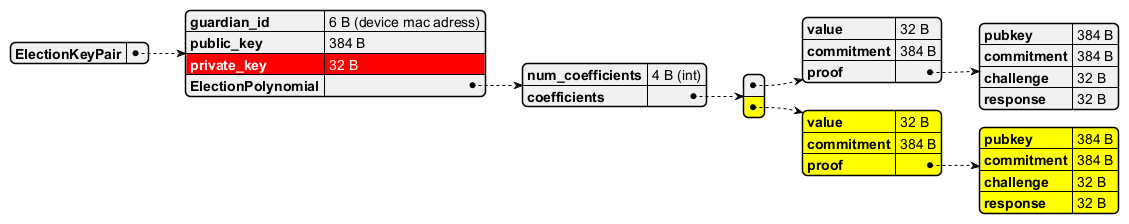
\includegraphics[width=1\textwidth]{abbildungen/Diagramme/mElectionKeyPair.png}
    \caption{ElectionKeyPair Message Definition}
    \label{Fig:keypair}
\end{figure}

\begin{figure}
    \centering
    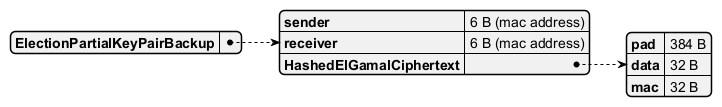
\includegraphics[width=1\textwidth]{abbildungen/Diagramme/mElectionPartialKeyPairBackup.png}
    \caption{ElectionKeyPairBackup Message Definition}
    \label{Fig:backup}
\end{figure}

\begin{figure}
    \centering
    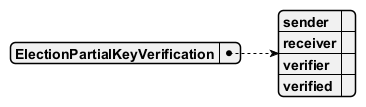
\includegraphics[width=1\textwidth]{abbildungen/Diagramme/mElectionPartialKeyVerification.png}
    \caption{mElectionPartialKeyVerification Message Definition}
    \label{Fig:verification}
\end{figure}


\subsection{Available Communication Protocols on the ESP32}
The ESP32 supports the wireless communication protocols Wi-Fi and Bluetooth. The Bluetooth system can be divided into Classic Bluetooth and Bluetooth Low Energy. Two hosts stacks are supported: Bluedroid and NimBLE. The Bluedroid based stack supports Bluetooth and Bluetooth Low Energy. The NimBLE based stack supports Bluetooth Low Energy only. For Bluetooth Low Energy-only usecases, using NimBLE is recommended as it requires less heap and flash size. \cite{esp-prog} \cite{esp-faq}. The Bluetooth Low Energy stack also supports Mesh Networking. Mesh networking enables many-to-many device communications and is optimized for creating large-scale device networks.\cite{esp-prog}

The Wi-Fi stack additionally supports Mesh Networking and Wi-Fi Neighbor Awareness Networking (NAN). NAN allows direct device-to-device communication and does not require any Internet or Access Point connection. \cite{esp-prog}. The ESP32 also supports the proprietary Wi-Fi communication protocol ESP-NOW which allows for connectionless communication between ESP32 devices. \cite{esp-prog}.Both Wi-Fi and Bluetooth can coexist but would requires time sharing control. Thus one protocol should be choosen.

The throughput of the wireless communication protocols depend on various factors such as environmental interference, connection interval, MTU size. The maximum MTU size for ESP32 Bluetooth LE is 517 bytes, for Classic Bluetooth is almost double 1008 bytes, and for Wi-Fi is 1500 bytes. The actual amount of data transmitted by the application layer will be slightly less than the MTU size due to header information. \cite{esp-faq}. The maximum throughput of ESP32 Bluetooth LE is about 90 KB/s, for Classic Bluetooth is about 200 KB/s, and for Wi-Fi is about 20 MBit/s TCP and 30 MBits/ UDP. \cite{esp-prog} \cite{esp-faq}.



At the uppermost layer of each communication protocol is the application layer. Own applications can be build on top of the Bluetooth Classic, Bluetooth Low Energy, or Wi-Fi stack. ESP-IDF supports the Application Layer protocols MQTT, HTTP, HTTPS, and Websocket protocols. \cite{esp-prog}.



Bluetooth Low Energy has a lower range than Bluetooth Classic. \cite{esp-faq}. The ESP32 supports the following communication protocols: Wi-Fi, Bluetooth Classic, Bluetooth Low Energy, and ESP-NOW. The ESP32 supports the following application layer protocols: MQTT, HTTP, HTTPS, and Websocket. \cite{esp-prog}.


\begin{comment}
    Add why this might be important
    What is difference between BLE
\end{comment}


\subsection{serialization}




For example, the Python implementation initially used a base-64 encoding of cryptographic values into JSON strings, which was problematic for the C++ implementation. 
This lead to a less efficient hexadecimal encoding. Later on, the Kotlin implementation supported Google’s Protocol Buffers, for an efficient binary representation, while the Rust code supported MongoDB’s BSON (a binary variant of JSON). 

The initial under-specification of how inputs to the cryptographic hash function should be seri-alized in the original version 1.0 specification has created unnecessary complications for achieving compatible implementations 

\cite[23-24]{eg-paper}


Communication: protobuf for serialization



\section{Usability}

Graphics Library: lvgl




Abkürzungen müssen im Abkürzungsverzeichnis angelegt werden.
Erste Verwendung einer \ac{ABK} jede weitere Verwendung der \ac{ABK}.

%Befehl um sämtliche Literatur im Literaturverzeichnis aufzuführen
\nocite{*}

